% !TEX program = xelatex
\documentclass[10pt,letterpaper,twocolumn]{article}
\usepackage[top=0.75in,bottom=0.75in,left=0.75in,right=0.75in]{geometry}
\usepackage{fontspec}
\usepackage{unicode-math}
\usepackage{xcolor}
\usepackage{booktabs}
\usepackage{tabularx}
\usepackage{array}
\usepackage{enumitem}
\usepackage{microtype}
\usepackage{graphicx}
\graphicspath{{assets/}{../arxiv-ac/figures/}}
\usepackage{caption}
\usepackage{tikz}
\usetikzlibrary{arrows.meta,positioning,shapes.geometric,fit}
\usepackage[most]{tcolorbox}
\usepackage{ragged2e}
\usepackage{natbib}
\usepackage{listings}
\usepackage{balance}
\usepackage{../ac-paper-layout}

\setmainfont{Latin Modern Roman}[Extension=.otf,UprightFont=lmroman10-regular,BoldFont=lmroman10-bold,ItalicFont=lmroman10-italic,BoldItalicFont=lmroman10-bolditalic]
\setsansfont{Latin Modern Sans}[Extension=.otf,UprightFont=lmsans10-regular,BoldFont=lmsans10-bold,ItalicFont=lmsans10-oblique,BoldItalicFont=lmsans10-boldoblique]
\setmonofont{Latin Modern Mono}[Extension=.otf,UprightFont=lmmono10-regular,ItalicFont=lmmono10-italic,Scale=0.85]
\definecolor{Pink}{RGB}{180,72,135}
\definecolor{Teal}{RGB}{120,80,180}
\definecolor{Purple}{RGB}{120,80,180}
\definecolor{Gold}{RGB}{156,112,20}
\definecolor{Green}{RGB}{40,125,82}
\definecolor{Red}{RGB}{180,58,66}
\definecolor{Ink}{RGB}{64,56,74}
\definecolor{Muted}{RGB}{119,119,119}
\definecolor{Pale}{RGB}{246,244,247}
\definecolor{PalePink}{RGB}{250,241,247}
\definecolor{PaleTeal}{RGB}{244,240,249}
\definecolor{Rule}{RGB}{214,209,218}

\hypersetup{pdfauthor={@jeffrey},pdftitle={No Paint 3.0: Human-Gated Generative Painting on Aesthetic Computer}}
\tolerance=900
\emergencystretch=1.2em

\newcolumntype{L}[1]{>{\RaggedRight\arraybackslash}p{#1}}
\newcolumntype{Y}{>{\RaggedRight\arraybackslash}X}
\newcommand{\mono}[1]{\code{#1}}
\newcommand{\shipped}{\textcolor{Green}{\textbf{SHIPPED}}}
\newcommand{\nexttag}{\textcolor{Gold}{\textbf{CONNECT NEXT}}}
\newcommand{\explore}{\textcolor{Purple}{\textbf{EXPLORE}}}

\newtcolorbox{hero}{colback=PalePink,colframe=Pink,boxrule=0.9pt,arc=2pt,left=10pt,right=10pt,top=8pt,bottom=8pt}
\newtcolorbox{note}{colback=PaleTeal,colframe=Teal,boxrule=0.65pt,arc=2pt,left=9pt,right=9pt,top=7pt,bottom=7pt}
\newtcolorbox{plain}{colback=Pale,colframe=Rule,boxrule=0.55pt,arc=2pt,left=9pt,right=9pt,top=7pt,bottom=7pt}

\tikzset{
  nodebox/.style={draw=Rule,rounded corners=2pt,fill=white,minimum height=0.34in,text width=0.95in,align=center,font=\scriptsize},
  pinkbox/.style={nodebox,draw=Pink,fill=PalePink},
  tealbox/.style={nodebox,draw=Teal,fill=PaleTeal},
  flow/.style={-{Latex[length=2.2mm]},line width=0.7pt,draw=Muted},
  feedback/.style={-{Latex[length=2.2mm]},line width=0.8pt,draw=Pink,dashed}
}

\begin{document}

\twocolumn[{%
\begin{center}

\includegraphics[height=4em]{pals.pdf}\par\vspace{0.45em}
{\acbold\fontsize{24pt}{28pt}\selectfont\color{acdark} No Paint 3.0}\par
\vspace{0.3em}
{\aclight\fontsize{11pt}{13pt}\selectfont\color{acpink} Human-Gated Generative Painting on Aesthetic Computer}\par
\vspace{0.55em}
{\normalsize\href{https://prompt.ac/@jeffrey}{@jeffrey}}\par
{\small\color{acgray} Aesthetic.Computer $\cdot$ ORCID: \href{https://orcid.org/0009-0007-4460-4913}{0009-0007-4460-4913} $\cdot$ 27 July 2026}\par
\vspace{0.45em}\rule{\textwidth}{1.5pt}
\end{center}
\begin{quote}
\small\noindent\textbf{Abstract.}
No Paint is a picture-making instrument organized around one perceptual decision: a system proposes a visual change, and a person presses \emph{No} to discard it or \emph{Paint} to preserve it. This paper specifies and reports the migration of that instrument into Aesthetic Computer (AC). The new conductor separates a transient proposal buffer from the accepted painting, records deterministic candidates and immutable decisions, reuses AC's brush, identity, storage, KidLisp, and sequencing systems, and connects a recovered archive of 32,184 anonymous paintings to contextual record pages and removal controls. It also defines several compatible human-in-the-loop paths: classic binary painting, manual Lisp juries, pairwise growth, and explicitly inferred---never falsely recovered---scores from finished rasters. A browser journey and Captutor/Frame evidence share one behavioral contract. A cross-machine performance facility adds frame-time, dropped-frame, long-task, commit-latency, and memory-soak receipts, with constrained-device runs on \mono{poorslice}. The central invariant remains human: generated code and remote search may propose, but only explicit acceptance mutates the painting or publishes a rule.
\end{quote}
\vspace{0.4em}
}]

\section{Introduction}

\textbf{The center stays human.} A machine proposes. A person perceives. \textbf{No} discards; \textbf{Paint / Yes / Yay} preserves. Basic brushes, KidLisp growth, visual inference, Merry sequencing, remote search, handles, uploads, tutorials, and archives supply, judge, remember, or continue that encounter. No Paint 3.0 treats that decision as a durable system boundary rather than merely a pair of buttons. As of revision \mono{4c4ba9448}, the living implementation includes the complete collision-free Construct visual vocabulary, fresh seeded substrates, timed unattended traversal, and a responsive full-surface decision interface.

\subsection{Context and related work}

The migration sits in three lineages. First, interactive evolutionary computation makes human evaluation the fitness function and identifies evaluator fatigue as a central constraint~\citep{sims1991,takagi2001}. No Paint uses a still narrower gesture: judge one live proposal in the context of the painting it would change. Second, AC grew from No Paint's community-authored brushes into a URL-addressed creative runtime~\citep{scudder2026ac}; KidLisp supplies a compact, inspectable language for generative descendants~\citep{scudder2026kidlisp}. Third, the repository's software archaeology treats source, exports, URLs, and observable behavior as distinct evidence rather than collapsing them into one origin story~\citep{scudder2026archaeology}. No Paint 3.0 therefore preserves the recovered instrument while making its state, decisions, provenance, and performance testable.

\begin{table*}[t]
\caption{Scope, evidence, and implementation-status vocabulary.}
\begin{tabularx}{\textwidth}{@{}L{1.12in}Y@{}}
\textbf{Artwork} & \emph{No Paint, 2016--present}; recovered Construct lineage plus a living Aesthetic Computer implementation. \\
\textbf{Version} & 3.0: AC owns proposal rendering, painting state, persistence, sharing, identity, and lineage. \\
\textbf{Evidence} & Repository implementation and tests; recovered 2021 source/export; 32,184 archived paintings; AC Merry, nopaint, KidLisp, handle, and storage systems. \\
\textbf{Status key} & \shipped\ exists now. \nexttag\ has an existing AC contract to wire. \explore\ is a deliberate possible UX path. \\
\end{tabularx}
\end{table*}

\section{Visual lineage: instrument to archive to living system}

\begin{figure*}[t]
\centering
\begin{minipage}[t]{0.49\textwidth}
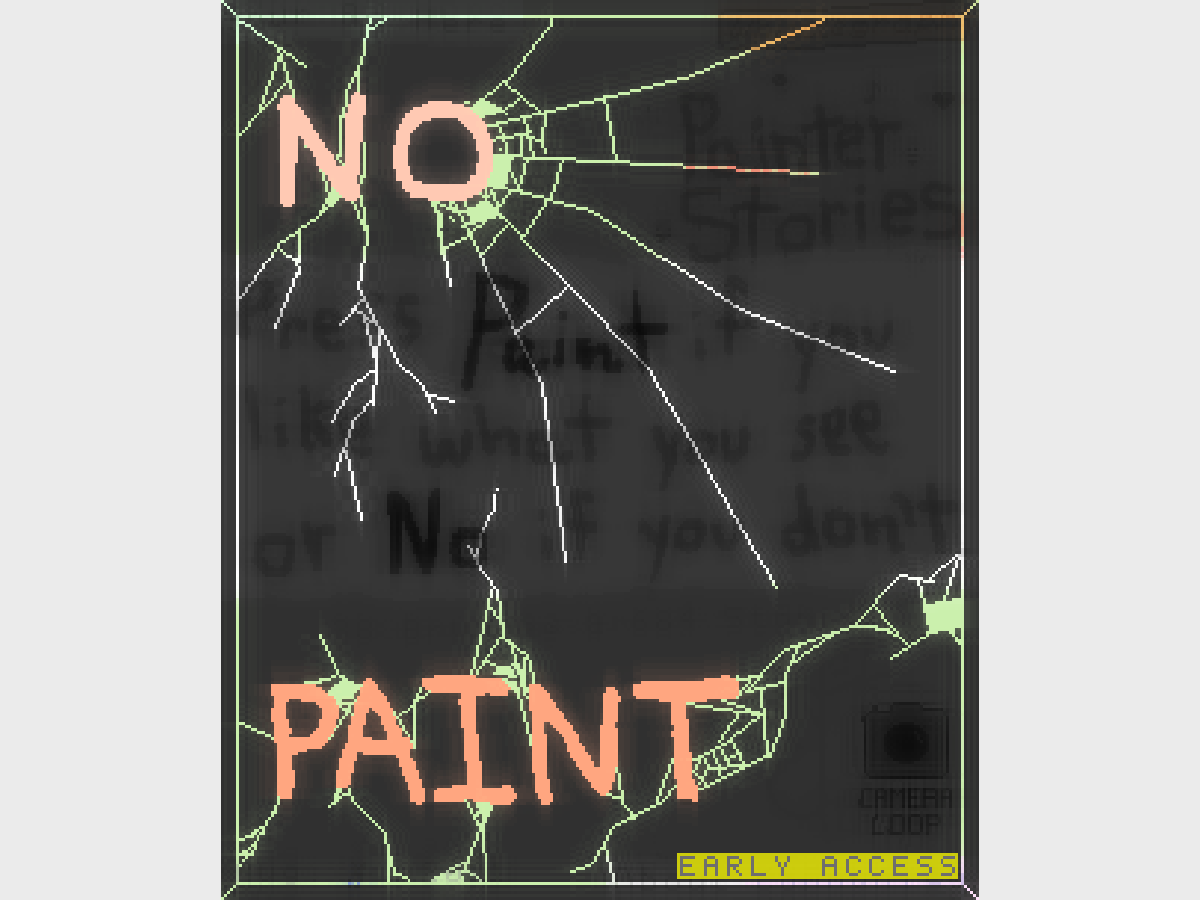
\includegraphics[width=\linewidth]{classic.png}
\caption*{\textbf{Classic instrument.} The preserved 2021 Construct export at \mono{nopaint.art/classic}: image-making is organized around the large hand-drawn No/Paint decision language.}
\end{minipage}\hfill
\begin{minipage}[t]{0.49\textwidth}
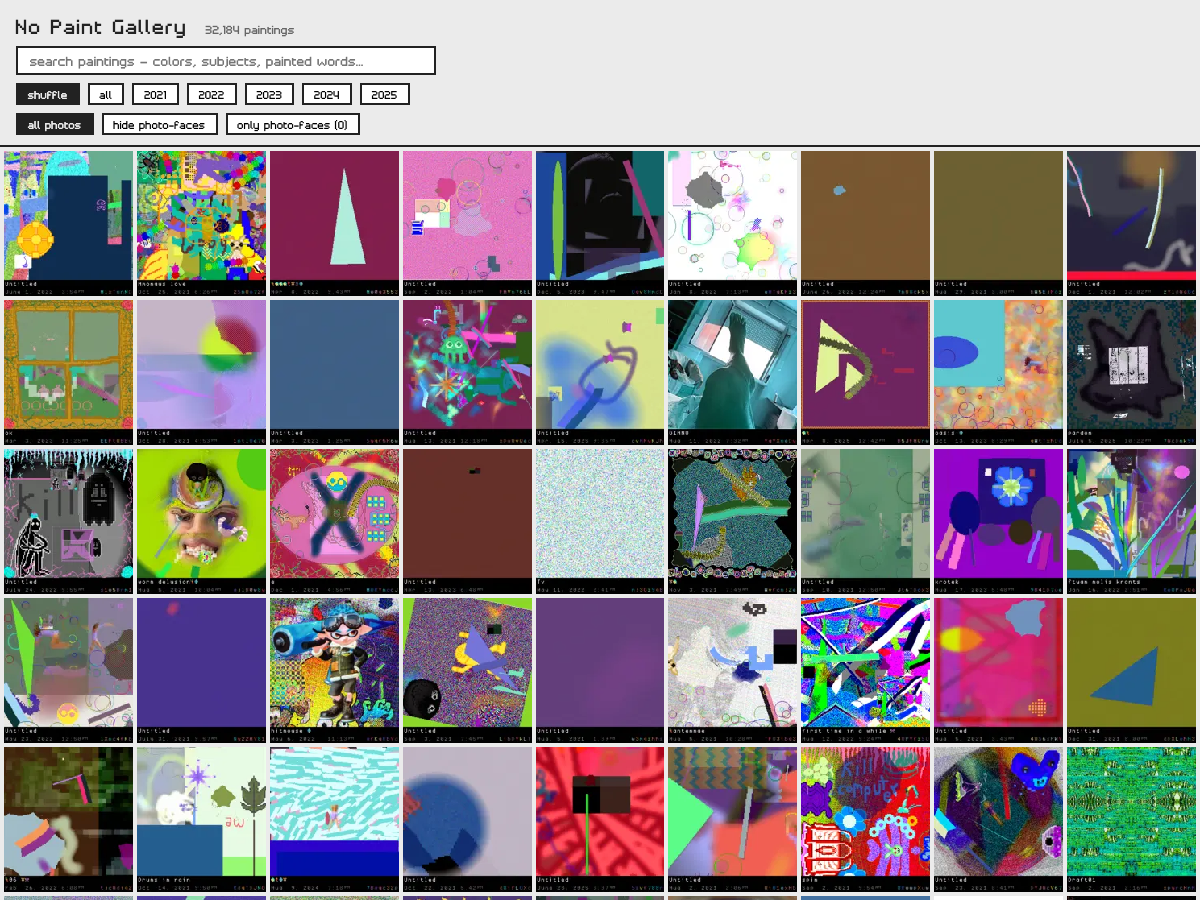
\includegraphics[width=\linewidth]{gallery.png}
\caption*{\textbf{Archive as public memory.} The searchable gallery exposes the accumulated field of 32,184 saved paintings with year and text/vision metadata.}
\end{minipage}
\caption{The recovered interface and archive at their native 4:3 aspect ratio. The classic canvas-to-controls proportion is treated as an interface constraint for 3.0, not as decoration.}
\end{figure*}

These are not mood-board references; they are live surfaces from the recovered system. The classic view establishes the interaction vocabulary and visual identity. The gallery demonstrates that repeated private decisions became a multi-year public body of work. No Paint 3.0 connects those histories to AC's state, identity, code, test, and publishing systems without erasing the older instrument.

\section{One loop, many intelligences}

\begin{figure*}[t]
\centering
\resizebox{0.88\textwidth}{!}{%
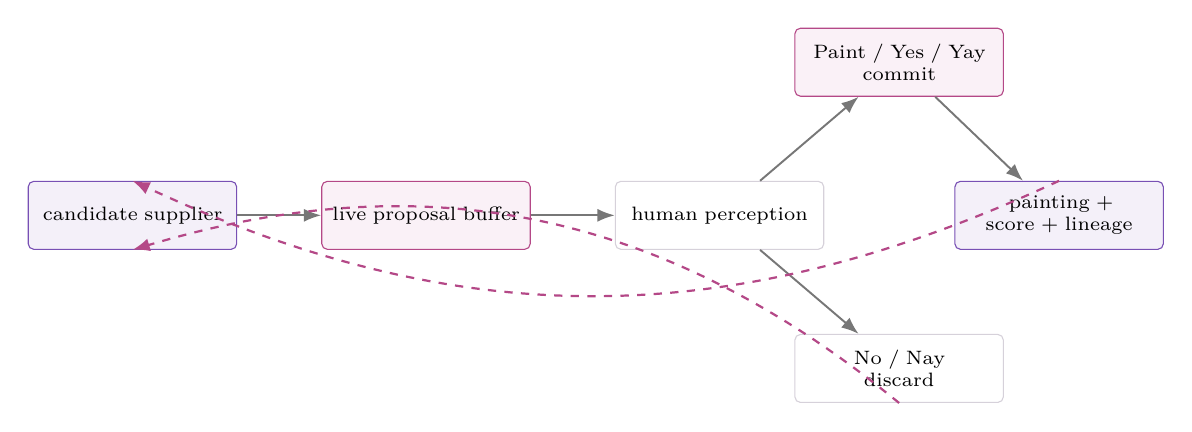
\begin{tikzpicture}[node distance=0.42in and 0.42in]
\node[tealbox] (supplier) {candidate supplier};
\node[pinkbox,right=of supplier] (proposal) {live proposal buffer};
\node[nodebox,right=of proposal] (human) {human perception};
\node[nodebox,below right=0.42in and -0.15in of human] (no) {No / Nay\\discard};
\node[pinkbox,above right=0.42in and -0.15in of human] (yes) {Paint / Yes / Yay\\commit};
\node[tealbox,right=0.65in of human] (lineage) {painting + score + lineage};
\draw[flow] (supplier)--(proposal);
\draw[flow] (proposal)--(human);
\draw[flow] (human)--(no);
\draw[flow] (human)--(yes);
\draw[flow] (yes)--(lineage);
\draw[feedback] (no.south) to[bend right=28] (supplier.south);
\draw[feedback] (lineage.north) to[bend left=25] (supplier.north);
\end{tikzpicture}
}
\caption{The invariant proposal--judgment--lineage loop. Candidate suppliers may change; explicit human acceptance remains the only mutation gate.}
\end{figure*}

Candidate suppliers are interchangeable. The decision contract is not.

\begin{table*}[t]
\caption{Candidate suppliers and their relationship to the decision contract.}
\begin{tabularx}{\textwidth}{@{}L{1.55in}L{1.0in}Y@{}}
\toprule
\textbf{Supplier} & \textbf{State} & \textbf{What it proposes} \\
\midrule
AC 3.0 catalog & \shipped & Deterministic Box, Ellipse, Line, Wipe, Camera, Softy, Bubbles, Grid Worm, Walker, Banner, and Wafer operations. \\
Basic AC brushes & \nexttag & Ordinary \mono{system = "nopaint"} pieces with their existing boot/paint/act/bake behavior and parameter vocabulary. \\
KidLisp rule queue & \nexttag & User-authored or machine-grown programs rendered into an isolated proposal surface. \\
Merry pipeline & \nexttag & Ordered, preloaded, timed, URL-addressable sequences; optionally crossfaded and UTC-synchronized. \\
Painting interpreter & \explore & Several honest coded readings inferred from a finished raster---never a false claim of original source recovery. \\
\mono{jastow} search & \explore & Bounded population growth, rendering, ranking, and mutation; never canonical storage or required live infrastructure. \\
\bottomrule
\end{tabularx}
\end{table*}

\section{What has been built}

\begin{table*}[t]
\caption{Implemented layers at the time of writing.}
\begin{tabularx}{\textwidth}{@{}L{1.65in}Y@{}}
\toprule
\textbf{Layer} & \textbf{Current implementation} \\
\midrule
Recovered lineage & Complete editable Construct project recovered and hash-verified; 2021 export served at \mono{nopaint.art} and preserved for \mono{/classic}. \\
Archive & 32,184 paintings from 2021--2025 indexed; searchable gallery with CDN thumbnails and visual descriptions. \\
Native conductor & Explicit choosing, proposing, committing, discarding, and paused states over AC's separate proposal buffer and persistent painting. \\
Determinism & Seeded weighted selection; a session URL can describe a repeatable score. Recovered weighting includes duplicated Box, Softy 1.5, and rare Walker 0.2. \\
Decision record & \mono{nopaint:session} stores version, seed, proposal number, operation, and No/Paint decisions alongside the local AC painting. \\
Migration ledger & All 38 recovered picker entries are inventoried. Twenty-nine collision-free visual operations render natively: 16 drawing contracts and 13 pixel transforms. Seven exact AC name collisions remain owned by AC; Load and Playlist remain controls. \\
Testing/tutorial spine & Unit contract, browser journey, optional native Frame receipts, and a fail-closed Captutor first-painting screenplay have been scaffolded. \\
\bottomrule
\end{tabularx}
\end{table*}

\begin{note}
\textbf{Already credible as an artwork.} The recovered source, multi-year public archive, playable classic, gallery, native proposal loop, and decision score establish continuity. Feature parity, user sync, and the broader Lisp ecology remain implementation work.
\end{note}

\subsection{The implemented 3.0 loop, as tested}

\begin{figure*}[t]
\centering
\begin{minipage}[t]{0.315\textwidth}
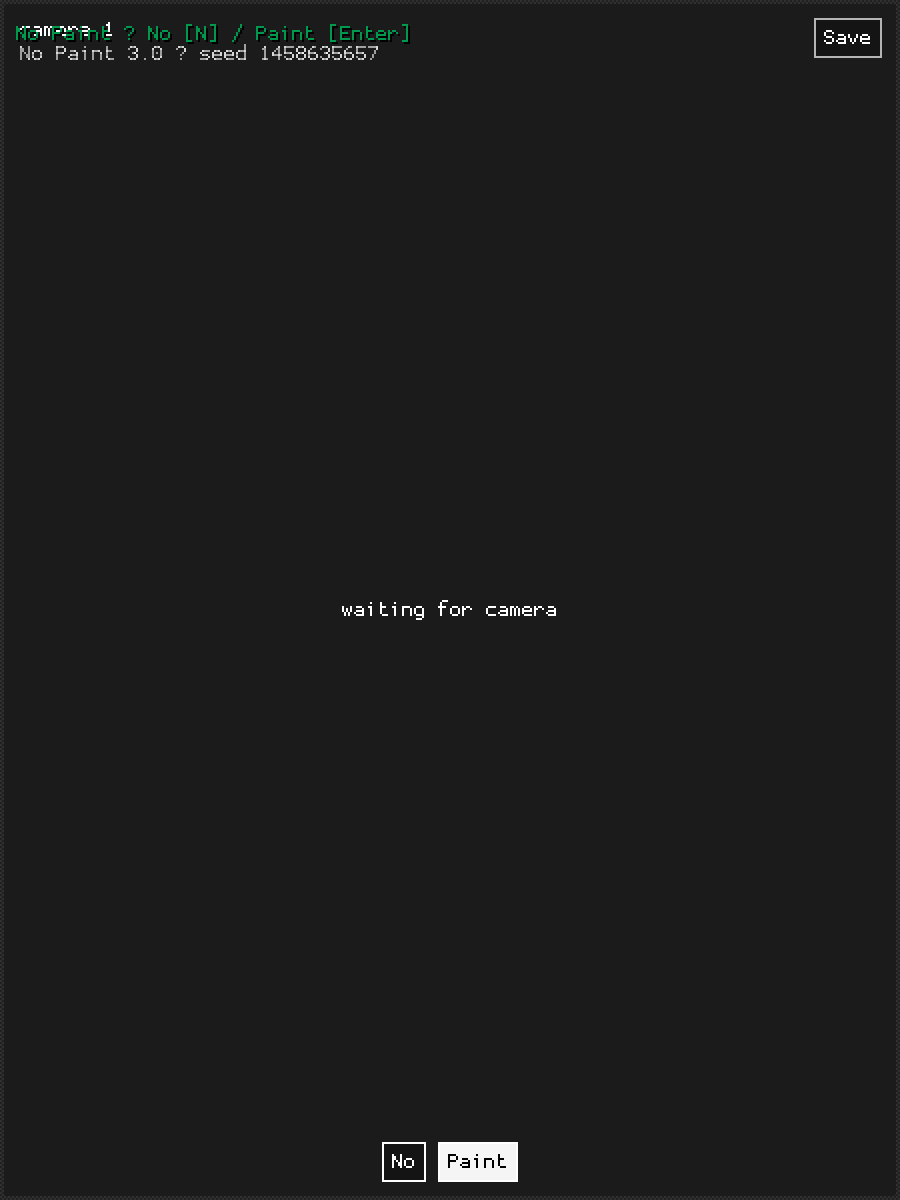
\includegraphics[width=\linewidth]{ac-3-first-proposal.png}
\caption*{\textbf{1. Propose.} A seeded operation animates only in the temporary proposal buffer.}
\end{minipage}\hfill
\begin{minipage}[t]{0.315\textwidth}
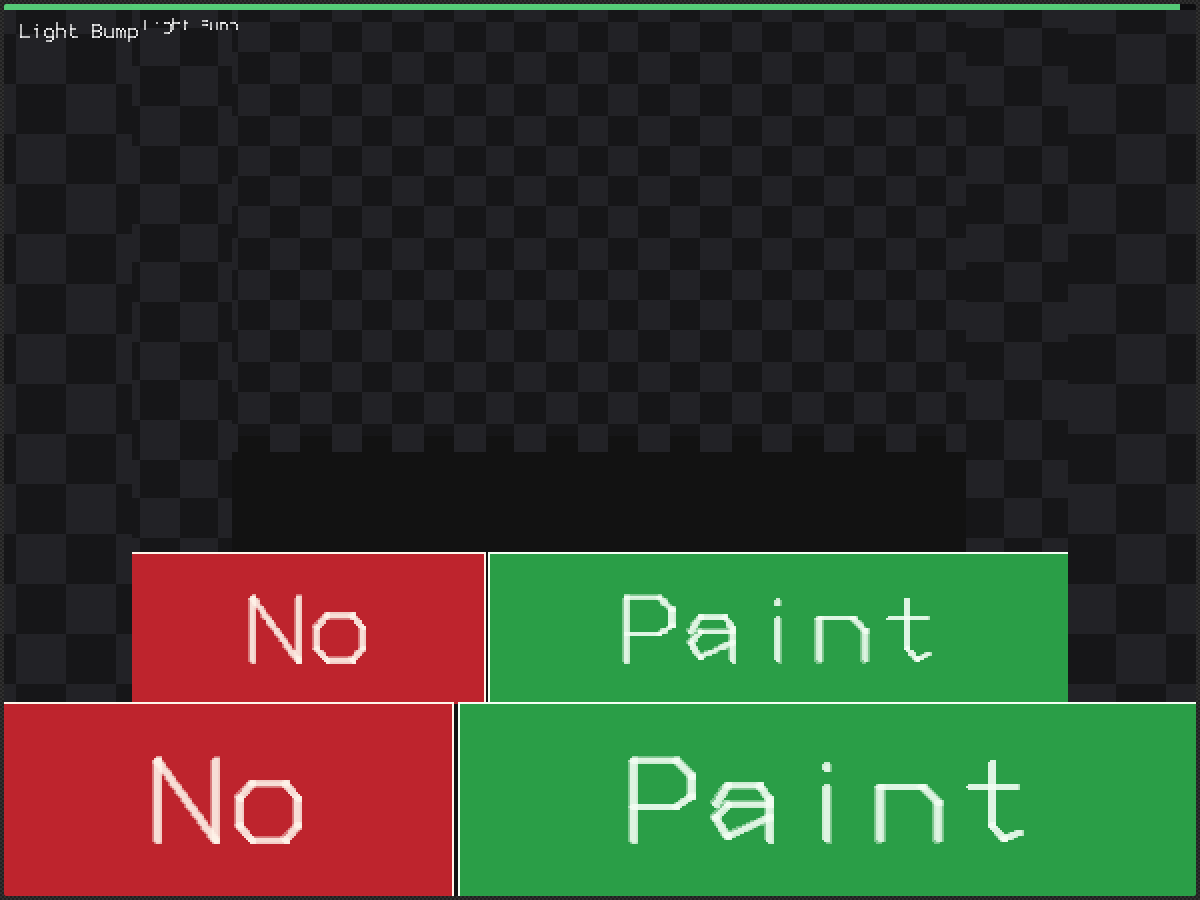
\includegraphics[width=\linewidth]{ac-3-after-no.png}
\caption*{\textbf{2. No.} The candidate is discarded; the accepted painting fingerprint is unchanged.}
\end{minipage}\hfill
\begin{minipage}[t]{0.315\textwidth}
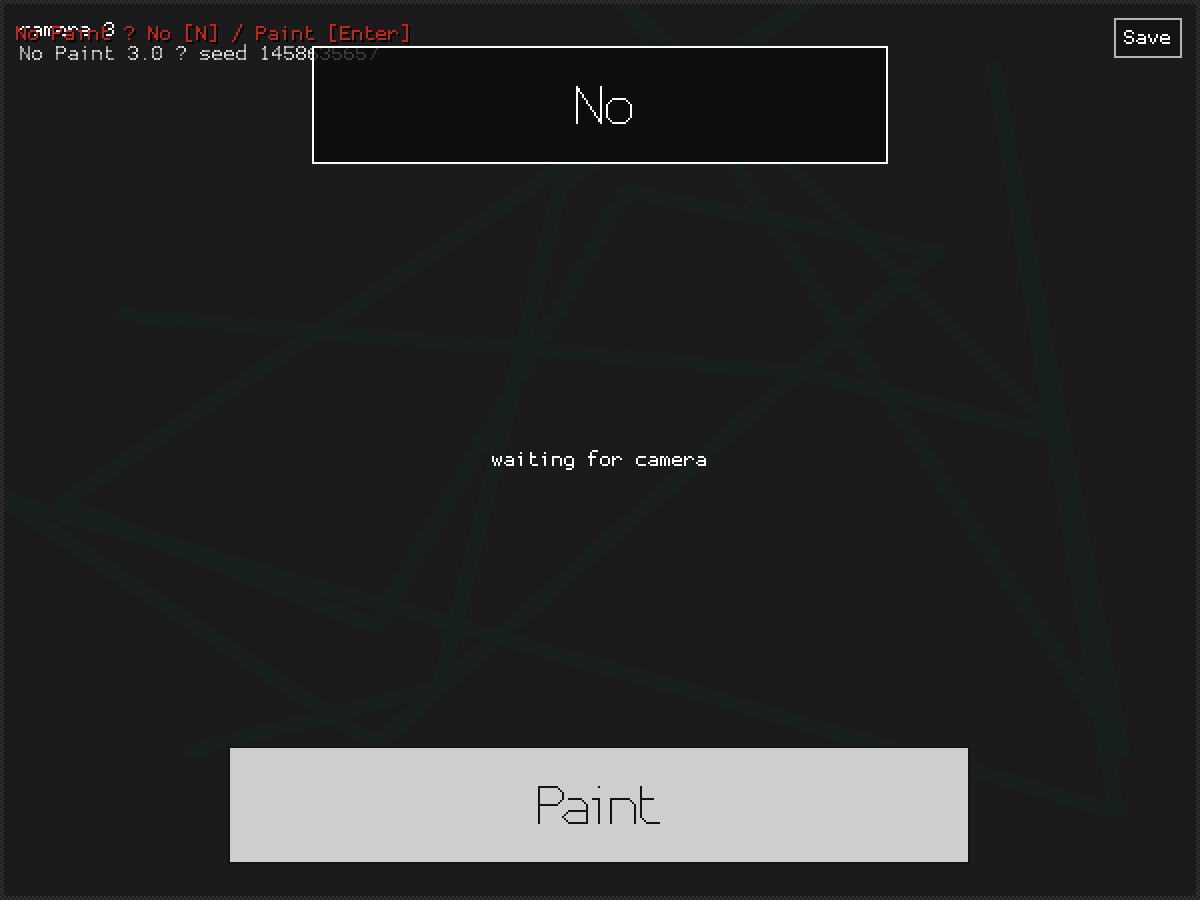
\includegraphics[width=\linewidth]{ac-3-after-paint.png}
\caption*{\textbf{3. Paint.} Pixels commit atomically, an undo point and score event persist, and the next proposal begins.}
\end{minipage}
\caption{Real-browser receipts from the canonical automated journey. The same behavioral contract drives the Captutor tutorial and optional native Frame evidence.}
\end{figure*}

\section{AC systems we should reuse}

\subsection{The existing nopaint system is the painting substrate}

Every basic brush can inherit \mono{system = "nopaint"}. The runtime supplies a persistent painting, transparent proposal buffer, coordinate transforms, pan/zoom, gesture recording, undo paintings, local database persistence, brush parameter parsing, robot input, present/bake behavior, and shared input handling.

The historical \mono{system.nopaint.no(api, yes)} operation is undo/redo over committed pixel snapshots. It must remain distinct from a proposal decision: \textbf{proposal No/Paint} judges a live candidate; \textbf{history back/forward} navigates already committed revisions. UI copy may say No/Yes, but internal events must not conflate them.

\begin{figure*}[t]
\centering
\resizebox{0.9\textwidth}{!}{%
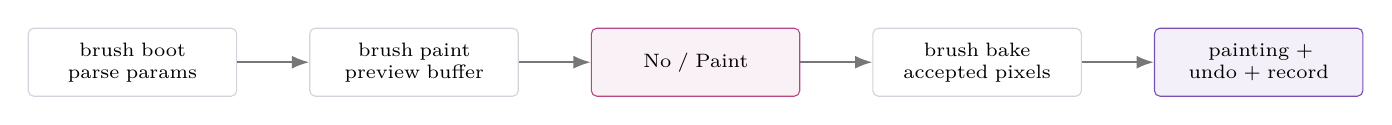
\begin{tikzpicture}[node distance=0.36in]
\node[nodebox] (boot) {brush boot\\parse params};
\node[nodebox,right=of boot] (paint) {brush paint\\preview buffer};
\node[pinkbox,right=of paint] (decision) {No / Paint};
\node[nodebox,right=of decision] (bake) {brush bake\\accepted pixels};
\node[tealbox,right=of bake] (store) {painting + undo + record};
\draw[flow] (boot)--(paint); \draw[flow] (paint)--(decision); \draw[flow] (decision)--(bake); \draw[flow] (bake)--(store);
\end{tikzpicture}
}
\caption{No Paint 3.0 conducts the existing AC nopaint substrate rather than introducing a second painting engine.}
\end{figure*}

\textbf{Rule:} No Paint 3.0 should be a conductor over this system, not a second painting engine. Basic brushes remain normal AC pieces; the conductor adapts their preview and bake into explicit proposals.

\subsection{Merry is the sequencing substrate}

Merry already parses duration-wrapped pieces, expands named bags, preloads modules, aligns playback to UTC, exposes current index/progress, advances steps, loops, stops cleanly, records tape, and can host KidLisp crossfades without jumping pieces. No Paint needs its sequencing ideas, but not automatic acceptance.

\begin{plain}
\textbf{Adaptation:} replace Merry's timer-only transition with a \emph{review gate}. A candidate can animate for a bounded preview; No/Paint advances immediately. Optional auto-step can advance undecided candidates as \textbf{Skip}, never as acceptance. The progress bar becomes a lineage/population bar.
\end{plain}

\section{The UX family}

These are modes over one event model, not competing product definitions.

\begin{table*}[t]
\caption{Compatible interaction paths over one event model.}
\begin{tabularx}{\textwidth}{@{}L{1.40in}L{1.15in}Y@{}}
\toprule
\textbf{Path} & \textbf{Decision} & \textbf{Experience} \\
\midrule
Classic No Paint & No / Paint & A live operation animates over the current painting; Paint commits pixels and asks again. \\
Lisp jury & Nay / Yay & One rendered KidLisp rule at a time; human perception supplies clean binary fitness. \\
Pairwise garden & Left / Right & Two mutations render from the same seed; choose which survives. \\
Rule studio & Reject / Accept / Edit & Code, render, parents, and parameters remain visible; accepted code becomes user-owned source. \\
Merry review & No / Yes / Step & Traverse a bag/population manually; previous/next/skip never alter the painting unless explicitly accepted. \\
Painting reading & Nay / Yay & A finished raster yields several compact coded interpretations; the participant curates the reading. \\
Autonomous growth & Interrupt / Judge & Remote compute evolves between visits, but pauses at meaningful perceptual forks. \\
Curatorial grid & Keep / Remove / Compare & Rapid review outside a painting; selections seed later No Paint sessions. \\
Teaching mode & Explain / Continue & Show how a rule, render, mutation, and decision relate; the same journey becomes a tutorial test. \\
\bottomrule
\end{tabularx}
\end{table*}

\section{Canonical state and events}

\subsection{Session}

\begin{lstlisting}[basicstyle=\ttfamily\scriptsize,breaklines=true]
NoPaintSession {
  id, version, ownerSub?, ownerHandle?, seed,
  mode, state, currentCandidateId?, currentStep,
  basePaintingHash, acceptedPaintingHash,
  createdAt, updatedAt, visibility
}
\end{lstlisting}

\subsection{Candidate}

\begin{lstlisting}[basicstyle=\ttfamily\scriptsize,breaklines=true]
Candidate {
  id, kind: brush | kidlisp | transform | inferred,
  source, sourceHash, renderSeed, runtimeVersion,
  parameters, parentIds[], generation?, supplier,
  sourcePaintingHash?, previewArtifact?, createdAt
}
\end{lstlisting}

\subsection{Immutable event stream}

\begin{lstlisting}[basicstyle=\ttfamily\scriptsize,breaklines=true]
NoPaintEvent {
  id, sessionId, sequence, at,
  type: proposed | no | paint | yay | nay | skip |
        step-forward | step-back | edit | save | publish,
  candidateId?, paintingBeforeHash?, paintingAfterHash?,
  actorSub?, actorHandle?, input: key | pointer | touch | voice | robot
}
\end{lstlisting}

The event stream is the artwork's score. Current state is a projection. Uploads are idempotent by \mono{sessionId + sequence}; local-first queues retry after reconnection. Pixels and large artifacts live in object storage; Mongo documents retain ownership, hashes, source, lineage, decisions, and URLs.

\begin{plain}
\textbf{Reducer boundary.} Input surfaces dispatch events; one reducer/effect layer owns state. Commit is atomic: candidate + before fingerprint $\rightarrow$ composite and flatten $\rightarrow$ undo snapshot, persist, and cross-tab broadcast $\rightarrow$ after fingerprint $\rightarrow$ append decision $\rightarrow$ clear overlay $\rightarrow$ request next. Reject clears only the overlay and never changes canvas revision, fingerprint, or history.
\end{plain}

\begin{hero}
\textbf{Core safety rule.} Remote growth and visual inference may propose candidates. Only an explicit human acceptance event may mutate the accepted painting or publish a user-owned rule.
\end{hero}

\section{Identity, handles, and ownership}

The first encounter must remain playable without registration. Account creation becomes meaningful at the moment a person wants continuity, public authorship, or cross-device growth.

\begin{figure*}[t]
\centering
\resizebox{0.92\textwidth}{!}{%
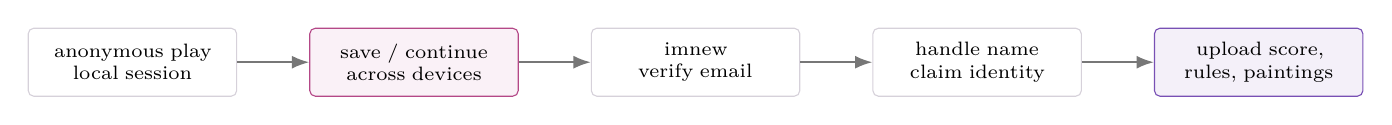
\begin{tikzpicture}[node distance=0.36in]
\node[nodebox] (anon) {anonymous play\\local session};
\node[pinkbox,right=of anon] (save) {save / continue\\across devices};
\node[nodebox,right=of save] (new) {\mono{imnew}\\verify email};
\node[nodebox,right=of new] (handle) {\mono{handle name}\\claim identity};
\node[tealbox,right=of handle] (sync) {upload score, rules, paintings};
\draw[flow] (anon)--(save); \draw[flow] (save)--(new); \draw[flow] (new)--(handle); \draw[flow] (handle)--(sync);
\end{tikzpicture}
}
\caption{Identity is invited at the continuity boundary, never required for the first perceptual decision.}
\end{figure*}

\begin{itemize}
  \item Anonymous sessions persist locally and can export a portable bundle.
  \item After authentication, queued events attach to the stable user subject; a handle supplies public attribution.
  \item Handle creation is never required to say No or Paint. It is invited when authorship has something worth naming.
  \item Public rule pages can live at handle-addressed AC routes; private sessions remain private by default.
  \item Publishing records source/runtime hashes so a visible render can always be traced to its code and score.
\end{itemize}

Existing AC contracts make this concrete:

\begin{itemize}
  \item \mono{imnew} calls the existing signup/login flow; \mono{handle name} claims a unique, verified-email handle through the authenticated \mono{/handle} backend. Ownership binds to immutable user subject, never to the mutable public handle.
  \item The common \mono{upload(...)} pipeline stores a PNG, calls authenticated \mono{/api/track-media}, returns the painting code, and already connects profile/ATProto records.
  \item Accepted public Lisp can use authenticated \mono{/api/store-kidlisp}; source-hash dedup means it is a publication store, not the authoritative decision ledger.
  \item Add one dedicated authenticated \mono{/api/nopaint-sessions} endpoint and collection for idempotent session/step sync. Keep pixel buffers out of Mongo; reference painting codes and Lisp codes.
\end{itemize}

Saving therefore has four explicit levels: \textbf{local checkpoint}, \textbf{cloud session sync}, \textbf{published painting}, and \textbf{published Lisp organism}. Only the last two should emit public profile events.

\section{Archive records, ownership, privacy, and removal}

The historical archive contains 32,184 anonymous paintings saved between 2021 and 2025. Each index slug should resolve to a stable human-readable record at \mono{nopaint.art/SLUG}, not directly to an uncontextualized PNG. The record presents the image, archive id, save date, machine-generated description and tags, privacy-review status, provenance limits, original file, and a prominent flag/removal route. Gallery thumbnails link to these records.

\begin{table*}[t]
\caption{Archive ownership, privacy, and removal conclusions.}
\begin{tabularx}{\textwidth}{@{}L{1.35in}Y@{}}
\toprule
\textbf{Question} & \textbf{Current conclusion and product rule} \\
\midrule
What AC owns & The No Paint software, brand, domain, storage infrastructure, archive compilation, metadata work, and aggregate curatorial presentation. \\
Individual image rights & Anonymous saving and archive custody do not by themselves prove a complete copyright assignment for every individual painting. Do not present that uncertainty as settled ownership. \\
Personal data & A camera-derived image, recognizable face, painted name, signature, location clue, or other identifying content can create a privacy interest even when the record has no account or handle. \\
Removal standing & A person may flag privacy, personal safety, a minor, accidental capture, personal information, creator interest, or another rights concern without first proving copyright ownership. \\
Data minimization & A removal request asks for archive id, reason, and only enough contact information to reply. Do not publish the request or require an account. Preserve a minimal private review/audit receipt. \\
\bottomrule
\end{tabularx}
\end{table*}

\begin{plain}
\textbf{Audit finding, 2026-07-27:} the gallery contains a photo-face moderation interface, and its descriptions visibly include selfie/person records, but the published 32,184-item manifest currently marks \textbf{zero} records as \mono{unsafe}. Therefore the archive-wide face/privacy test is \textbf{not complete}. Until a documented detector plus human review has run, every unflagged record must say ``archive-wide face/privacy review pending,'' never ``cleared.''
\end{plain}

Recommended review states are \mono{pending}, \mono{machine-flagged}, \mono{human-review}, \mono{restricted}, \mono{removal-requested}, \mono{removed}, and \mono{cleared-with-date}. A face detector is a triage aid, not a privacy verdict: false negatives are expected, stylized or embedded photos may evade detection, and non-face personal data still matters. Default public behavior should blur/restrict strong photographic-person matches pending review; removed records retain only a non-public minimal tombstone sufficient to prevent accidental re-publication.

\subsection{What one anonymous user-data record actually contains}

\begin{figure*}[t]
\centering
\begin{minipage}[t]{0.28\textwidth}
\centering

\includegraphics[width=\linewidth]{archive-l4f0ipzy.png}
\caption*{\textbf{Archived PNG.} The upper 256-by-256 field is the painting; the historical app baked title, local date/time, and stable id into a 32-pixel caption bar. This abstract record was selected to avoid knowingly reproducing a face while review remains incomplete.}
\end{minipage}\hfill
\begin{minipage}[t]{0.69\textwidth}
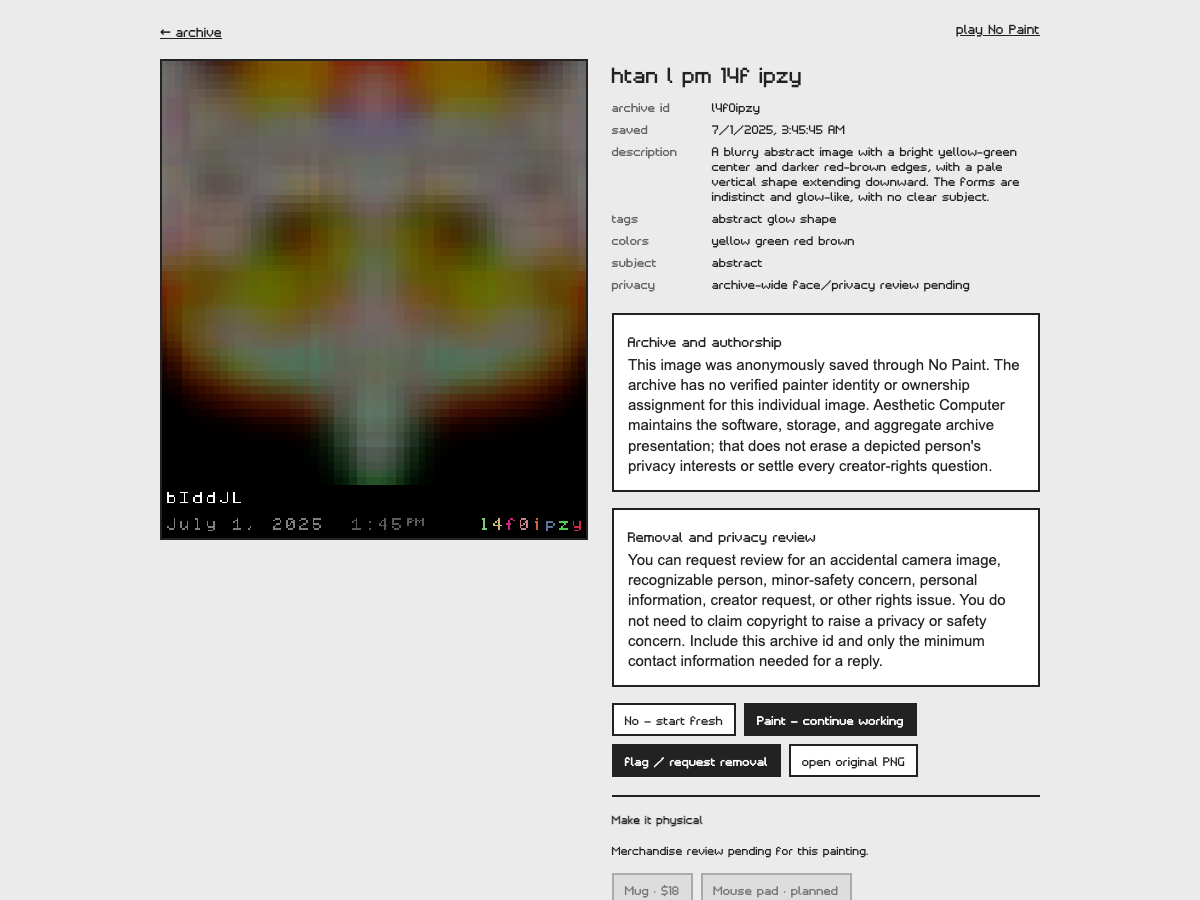
\includegraphics[width=\linewidth]{record.png}
\caption*{\textbf{Canonical record surface.} The live \mono{nopaint.art/l4f0ipzy} page joins image and id to save timestamp, OCR/title guess, machine description, tags, colors, subject class, privacy status, original file, removal contact, continuation actions, and merchandise eligibility.}
\end{minipage}
\caption{User data is presented with context and uncertainty rather than as a bare image. Generated descriptions are search aids, not author statements.}
\end{figure*}

\subsection{Continuation and productization}

Each record is a fork point. \textbf{No} opens a fresh deterministic canvas while retaining a private provenance note that the archive image was declined as a starting surface. \textbf{Paint} imports the top 256-by-256 artwork (not its baked caption bar), establishes it as the undo base, and carries archive id, record URL, image URL, and load status into the No Paint session. The displayed save date and derived metadata remain attached to the public record.

The existing AC mug checkout already supplies Stripe payment, Printful mockups, fulfillment, product records, and order recovery. Archive commerce reuses it through a strict manifest allowlist and the \mono{np-ID} image adapter; arbitrary remote URLs are never accepted. A record exposes purchase only when it has explicit \mono{merchEligible: true} after face/privacy and rights review. Missing or false means ``merchandise review pending.'' Removal must disable future checkout and discovery and remove cached product previews where appropriate.

The product ladder is \textbf{mug first}, then \textbf{standard mouse pad}, then \textbf{desk mat}; posters, framed prints, and stickers follow after the review workflow is operating. Mouse pads should use a generalized catalog record---product, variant, print geometry, placement, retail price, mockup, and eligibility---rather than a copied mug endpoint. Printful mockups are asynchronous and rate-limited, so generate on product intent and cache, never on every archive-page view.

\subsection{Complete UX path map}

\begin{figure*}[t]
\centering
\resizebox{\textwidth}{!}{%
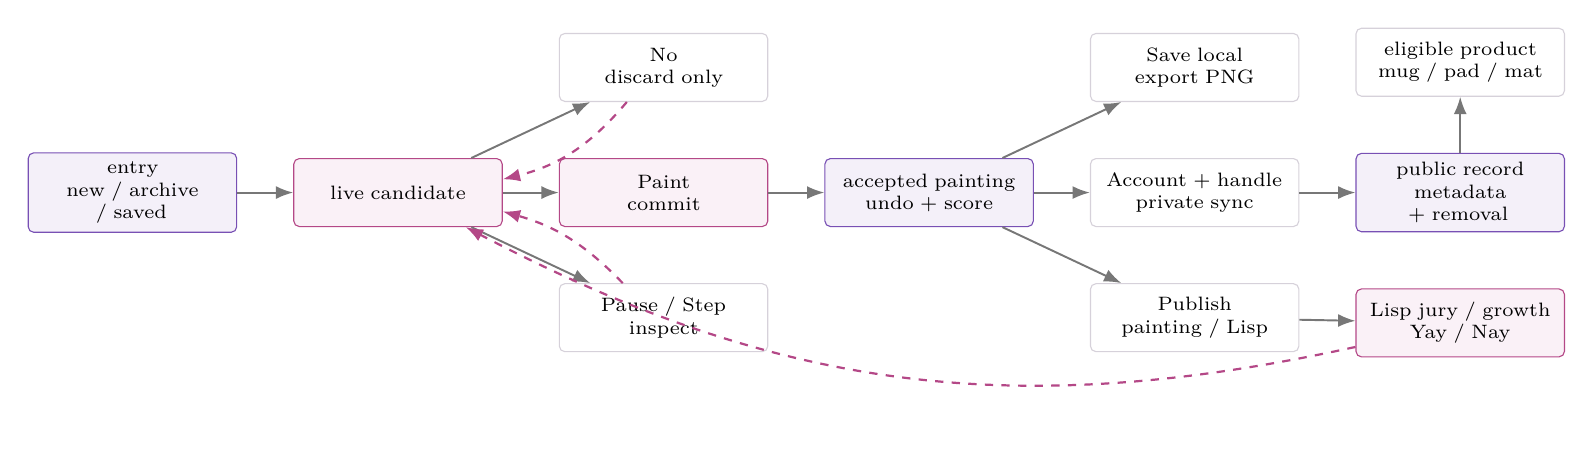
\begin{tikzpicture}[node distance=0.28in and 0.28in,every node/.append style={font=\footnotesize}]
\node[tealbox] (entry) {entry\\new / archive / saved};
\node[pinkbox,right=of entry] (candidate) {live candidate};
\node[nodebox,above right=of candidate] (no) {No\\discard only};
\node[pinkbox,right=of candidate] (paint) {Paint\\commit};
\node[nodebox,below right=of candidate] (pause) {Pause / Step\\inspect};
\node[tealbox,right=of paint] (accepted) {accepted painting\\undo + score};
\node[nodebox,above right=of accepted] (save) {Save local\\export PNG};
\node[nodebox,right=of accepted] (account) {Account + handle\\private sync};
\node[nodebox,below right=of accepted] (publish) {Publish\\painting / Lisp};
\node[tealbox,right=of account] (record) {public record\\metadata + removal};
\node[nodebox,above=of record] (product) {eligible product\\mug / pad / mat};
\node[pinkbox,below=of record] (grow) {Lisp jury / growth\\Yay / Nay};
\draw[flow] (entry)--(candidate); \draw[flow] (candidate)--(no); \draw[flow] (candidate)--(paint); \draw[flow] (candidate)--(pause);
\draw[flow] (paint)--(accepted); \draw[feedback] (no) to[bend left=18] (candidate); \draw[feedback] (pause) to[bend right=15] (candidate);
\draw[flow] (accepted)--(save); \draw[flow] (accepted)--(account); \draw[flow] (accepted)--(publish); \draw[flow] (account)--(record);
\draw[flow] (record)--(product); \draw[flow] (publish)--(grow); \draw[feedback] (grow) to[bend left=20] (candidate);
\end{tikzpicture}
}
\caption{End-to-end UX paths share one accepted-painting and immutable-event model. The diagram is deliberately full-width so nodes retain legible, non-overlapping proportions.}
\end{figure*}

\begin{table*}[t]
\caption{Journey promises and their required evidence.}
\begin{tabularx}{\textwidth}{@{}L{1.32in}Y@{}}
\toprule
\textbf{Path} & \textbf{Promise and evidence} \\
\midrule
First painting & Seeded proposal $\rightarrow$ No without mutation $\rightarrow$ Paint with mutation $\rightarrow$ pause/resume $\rightarrow$ PNG request. Browser-tested and mirrored by Captutor. \\
Archive continuation & Gallery $\rightarrow$ record $\rightarrow$ No/new or Paint/import $\rightarrow$ archive provenance retained. Real CDN import is browser-tested. \\
Account continuity & Anonymous local work $\rightarrow$ optional \mono{imnew} $\rightarrow$ verified handle $\rightarrow$ idempotent private session sync $\rightarrow$ deliberate publication. \\
Lisp jury & Candidate source + deterministic render $\rightarrow$ Yay/Nay/Skip/Previous/Next $\rightarrow$ accepted rule lineage; code stays inspectable and editable. \\
Painting reading & Finished raster $\rightarrow$ multiple inferred KidLisp responses $\rightarrow$ perceptual jury $\rightarrow$ one editable descendant, never false source recovery. \\
Products & Reviewed record $\rightarrow$ product choice $\rightarrow$ cached mockup $\rightarrow$ Stripe $\rightarrow$ Printful; removal/restriction blocks new checkout. \\
\bottomrule
\end{tabularx}
\end{table*}

\section{Painting to code, without pretending}

A raster cannot reveal one true source program. The product should call the result a \textbf{reading}, \textbf{response}, or \textbf{inferred score}.

\begin{figure*}[t]
\centering
\resizebox{0.9\textwidth}{!}{%
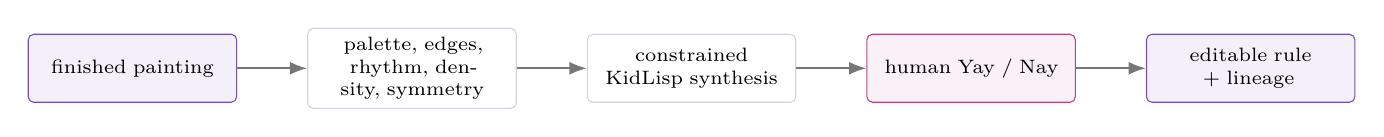
\begin{tikzpicture}[node distance=0.35in]
\node[tealbox] (raster) {finished painting};
\node[nodebox,right=of raster] (features) {palette, edges, rhythm, density, symmetry};
\node[nodebox,right=of features] (synth) {constrained KidLisp synthesis};
\node[pinkbox,right=of synth] (jury) {human Yay / Nay};
\node[tealbox,right=of jury] (organism) {editable rule + lineage};
\draw[flow] (raster)--(features); \draw[flow] (features)--(synth); \draw[flow] (synth)--(jury); \draw[flow] (jury)--(organism);
\end{tikzpicture}
}
\caption{A finished raster can seed an explicitly inferred, human-selected KidLisp descendant; it cannot reveal a unique original program.}
\end{figure*}

Deterministic vision supplies the initial structural sketch. A bounded synthesizer produces valid KidLisp. Render similarity can rank candidates, but perception chooses. The accepted rule can mutate, render at any resolution, and become a supplier for another painting.

\section{The role of jastow}

\mono{jastow} is an optional worker, not part of the artwork's availability path. At this writing it is offline on the Tailnet and was last seen two days ago, so the most recent Lisp growth results could not be audited for this report.

\begin{table}[h]
\caption{Division of responsibility between optional remote search and canonical AC behavior.}
\small
\begin{tabularx}{\linewidth}{@{}L{0.72in}Y@{}}
\toprule
\textbf{Do there} & Population mutation, batch KidLisp rendering, visual embeddings, bounded search, thumbnail/video generation, and offline evaluation. \\
\textbf{Do in AC} & Canonical compilation, sandboxed preview, user decision, painting mutation, identity, persistence, publishing, and cached offline playback. \\
\textbf{Never require} & A live SSH connection, residential workstation uptime, or unbounded generated code to play a saved session. \\
\bottomrule
\end{tabularx}
\end{table}

\section{Testing and tutorial production are one surface}

\subsection{Implementation update: 27 July 2026}

The production conductor now exposes 29 collision-free Construct-era visual operations. The drawing set is Aura, Banner, Breathe, Bubbles, Build, Caterpillar, Dark Window, Ellipse, Frame, Grid Worm, Rainbow, Softy, Triangle, Vignette, Wafer, and Walker. The pixel set is Contrast, Flip, Invert, Light Bump, Mirror, Quicksand, Recurse, Saturate, Scroll, Sharpen, Spin, Turn, and Zoom. Existing AC pieces retain the colliding names Blur, Box, Camera, Line, Noise, Stamp, and Wipe. Recovered constants, deterministic scores, primary audio cues, and fidelity classifications live in the migration ledger; approximations are named rather than represented as pixel-exact recovery.

The current surface fixes the No/Paint controls flush to the bottom, treats the entire region above them as one painting button, places the operation label at the screen's upper-left, and displays a thin five-second Merry countdown at the top edge. Undecided proposals advance as timeouts without fabricating a No or Paint event. Holding a decision or pausing freezes proposal time. The checker field moves only from its own simulation phase, never from mouse motion. Fresh launches accept \mono{?fresh=1}, \mono{nopaint fresh}, and \mono{/nopaint:fresh}; every genuinely new canvas begins from a deterministic bounded noise rectangle, while resumed and archive-derived paintings retain their source pixels.

The browser journey covers fixed logical resolution under responsive presentation, No without mutation, Paint with mutation, sliding between decisions, key-up cancellation, pause/resume, whole-surface completion, in-place upload, code receipt, and fresh restart. Invert's initial failure was traced to a queued buffer wipe executing after direct pixel mutation; transform buffers now avoid that ordering hazard and static transform pixels upload once per proposal. Cursor repaint now follows vertical and subpixel movement as well as horizontal movement. Functional journeys are green. Blueberry measurements have alternated between approximately 61 and 30 presented frames per second with no Long Tasks, so the remaining performance task is to isolate display/compositor cadence and obtain the designated headed Poorslice trace rather than treating either local number as universal evidence.

Every canonical journey should exist twice from one behavioral contract:

\begin{enumerate}
  \item A fast real-browser e2e asserts the read-only No Paint state hook, painting fingerprints, decision sequence, animation freeze, persistence, and PNG delivery.
  \item A Captutor screenplay performs the same journey with narration, visible cursor intent, opening/closing cards, and required evidence checks.
  \item Frame captures the actual macOS display at milestones, including browser chrome, clipping, cursor, OCR, and compositor reality.
  \item The encoded tutorial emits a storyboard/QA receipt and fails closed when required evidence is missing.
\end{enumerate}

\subsection{Frame-rate and interaction budgets}

The test journey now writes a machine-readable \mono{performance.json} receipt. It samples real \mono{requestAnimationFrame} intervals during an animated proposal; reports achieved FPS, average/p50/p95/maximum frame time, frames over 33.3\,ms, Long Tasks over 50\,ms, JavaScript heap and heap delta where Chromium exposes them; and measures renderer-clock latency from the No or Paint key event to the next proposal. Strict mode targets sustained 60\,Hz behavior with a practical floor of 59.5\,fps, p95 frame time at or below 20\,ms, no frames over 33.3\,ms, no Long Tasks, and decision completion within 250\,ms. These are acceptance budgets, not claims about every device.

The instrumentation and strict assertions were exercised locally as a functional smoke test, but local Blueberry timings are deliberately not used as performance evidence. \mono{poorslice} is the designated profiling runner for the paper. It was offline and last seen four days earlier during this revision, so this draft reports the poorslice baseline as pending rather than substituting numbers from a different machine. A passing release receipt requires the headed browser and native Frame run to complete on poorslice; a portable headless pass alone is insufficient.

The follow-through matrix uses the same seed and journey across headed browser E2E, Captutor, Frame, and poorslice. Captutor supplies narrated intent and milestone timing; Frame verifies the actual macOS compositor surface; the browser receipt supplies high-resolution timing; and poorslice supplies a stable constrained host. Runs cover 640$\times$480, 1280$\times$720, and 1920$\times$1080; idle proposal, repeated No, repeated Paint, pause, save, and heavy suppliers; three warm samples plus a longer memory soak. Receipts must carry source revision, browser/OS, viewport and pixel ratio, power state where available, and raw trace paths.

\begin{plain}
\textbf{First canonical journey:} boot a reproducible proposal $\rightarrow$ No without mutation $\rightarrow$ Paint with mutation $\rightarrow$ pause/freeze $\rightarrow$ resume $\rightarrow$ save a PNG. Future journeys add handle creation, Lisp jury, pairwise growth, painting reading, and publishing.
\end{plain}

\section{Delivery sequence}

\begin{enumerate}
  \item \textbf{Stabilize the spine.} Finish the seeded browser e2e against the real AC boot shell; retain deterministic unit coverage and Captutor's static acceptance contract.
  \item \textbf{Adapt basic brushes.} Create a proposal adapter that runs existing nopaint brush preview/bake behavior without duplicating brush implementations.
  \item \textbf{Add manual Lisp jury.} Frozen fixture population first; Yay/Nay/Skip/Previous/Next; immutable local event log.
  \item \textbf{Sync to account.} Authenticated idempotent event upload, session list, handle attribution, private-by-default visibility, portable export.
  \item \textbf{Deepen authored parity.} The collision-free visual catalog is ported; next connect multi-cue audio timelines, exact compositor effects where AC supports them, stamps/profiles, playlists, and painter stories.
  \item \textbf{Connect growth.} Import recent \mono{jastow} experiment outputs, define a versioned candidate packet, and run bounded asynchronous generations with cached fallback.
  \item \textbf{Add painting readings.} Deterministic feature extraction, constrained KidLisp candidates, perceptual review, and explicit ``inferred from'' provenance.
  \item \textbf{Change the front door.} When 3.0 is credible and recoverable, route \mono{nopaint.art} to it; retain \mono{/classic}, \mono{/gallery}, and add \mono{/story}.
\end{enumerate}

\section{Launch definition}

No Paint 3.0 succeeds when:

\begin{itemize}
  \item A new person understands No/Paint in seconds without an account.
  \item The same piece works with keyboard, pointer, touch, voice, and robot inputs.
  \item Existing AC brushes can become proposals without forks.
  \item KidLisp candidates remain inspectable, editable, reproducible, and sandboxed.
  \item No/Yay/Nay/step changes survive locally, sync idempotently, and belong to a user account after optional handle creation.
  \item Every published painting connects to its score, accepted rules, runtime versions, and lineage.
  \item Offline play works without \mono{jastow}; remote compute enriches rather than controls the artwork.
  \item Each major UX path ships with a passing browser journey, Captutor tutorial, Frame evidence, and storyboard receipt.
\end{itemize}

\begin{hero}
\centering
{\large\bfseries Paintings become scores. Scores grow paintings.}\par
\vspace{3pt}
The machine can propose forever. The artwork happens where a person decides what survives.
\end{hero}

\balance
\section{Conclusion}

No Paint 3.0 is not defined by how many generators it can attach. It is defined by a legible proposal boundary, an explicit human mutation gate, and a score that lets a painting be continued, studied, tested, removed, or reinterpreted without inventing provenance. The migration now has a native conductor, archive records, deterministic journeys, and an executable performance receipt. Full brush parity, account sync, archive-wide privacy review, constrained-device profiling, and product eligibility remain staged work and are named as such.

\bibliographystyle{plainnat}
\bibliography{references}

\end{document}
